\subsection{Homological algebra in $\mathsf{Ab}(X)$}

We will now define the notion of injectivity and surjectivity for maps of sheaves. The categorification of injective mpas are monomorphisms, while surjective maps correspond to epimorphisms. Epimorphisms of sheaves are tricky and the reason why sheaf cohomology is a non-trivial invariant. The general frameworks in which to study (co-)homology are abelian categories. The notion of an abelian category is an abstraction of the category of abelian groups. Abelian categories are the general settings in which to do homological algebra.

\begin{definition}[Monomorphisms and Epimorphisms]
	Let $f: X \to Y$ be a morphism (in any category). We say that $f$ is a \textit{monomorphism} if $f \circ g_1 = f \circ g_2 \implies g_1 = g_2$.
	We say that $f$ is a \textit{epimorphism} if $g_1 \circ  f  = g_2 \circ f \implies g_1 = g_2$.
\end{definition}

\begin{proposition}[Monomorphisms in $\sh(C,J)$]
	Let $\varphi: F \to G$ be a morphism of sheaves on a site $(C,J)$. We say that $\varphi$ is injective if for each object $U$ of $C$, the map $\varphi: F(U) \to G(U)$ is injective.
\end{proposition}

\begin{proposition}[Epimorphisms in $\sh(C,J)$]
	A morphism of sheaves $\varphi: F \to G$ is an epimorphism in $\Sh(C,J)$ if and only if for every object $U$ and every section $s \in G(U)$ there exists a covering $\{U_i \to U\}$ such that the restriction $s|_{U_i}$ is contained in the image of $\varphi: F(U_i) \to G(U_i)$. We also say that \textit{$\varphi$ is locally surjective}.
\end{proposition}

\begin{proof}
	$(\implies)$ Suppose that $\varphi$ is locally surjective. For any object $U$ of $C$ and any $s \in G(U)$ choose a cover $\{f_i: U_i \to U\}$ as stated in the proposition. Let $\alpha_1, \alpha_2: G \to H$ be morphisms such that $\alpha_1 \circ \varphi = \alpha_2 \circ \varphi$. 
	\[
		% https://q.uiver.app/?q=WzAsMyxbMCwwLCJGIl0sWzEsMCwiRyJdLFsyLDAsIkgiXSxbMCwxLCJcXHZhcnBoaSJdLFsxLDIsIlxcYWxwaGFfMiIsMix7Im9mZnNldCI6MX1dLFsxLDIsIlxcYWxwaGFfMSIsMCx7Im9mZnNldCI6LTF9XV0=
		\begin{tikzcd}
			F & G & H
			\arrow["\varphi", from=1-1, to=1-2]
			\arrow["{\alpha_2}"', shift right=1, from=1-2, to=1-3]
			\arrow["{\alpha_1}", shift left=1, from=1-2, to=1-3]
		\end{tikzcd}\]
	We need to show that $\alpha_1 = \alpha_2$.  Now for each $f_i: U_i \to U$ and each section $s \in F(U)$ we have $(\alpha_1 \circ f_i)(s) = (\alpha_2 \circ f_i)(s)$ or equivalently  $\alpha_1(s)|_{U_i} = \alpha_2(s)|_{U_i}$. This means that $\alpha_1$ agrees with $\alpha_2$ for the cover $\{U_i\}$. Since $H$ is a sheaf it follows that $\alpha_1 = \alpha_2$.\par
	$(\impliedby)$ 
\end{proof}

\begin{definition}[Additive categories]
	An \textit{additive category} is a category $C$ with finite direct sums such that the sets $\Hom(A,B)$ have the structure of an abelian group 
\end{definition}

\begin{definition}[Kernels]
	Let $C$ be a category with an initial object $0$ and pullbacks. The kernel of a morphism $f: A \to B$ is the pullback
	\[
		% https://q.uiver.app/?q=WzAsNCxbMCwwLCJcXGtlciBmIl0sWzAsMSwiQSJdLFsxLDAsIjAiXSxbMSwxLCJCIl0sWzAsMV0sWzAsMl0sWzEsMywiZiIsMl0sWzIsM11d
		\begin{tikzcd}
			{\ker f} & 0 \\
			A & B
			\arrow[from=1-1, to=2-1]
			\arrow[from=1-1, to=1-2]
			\arrow["f"', from=2-1, to=2-2]
			\arrow[from=1-2, to=2-2]
		\end{tikzcd}.
	\]
	If $C$ is enriched over abelian groups, meaning that $\Hom(A,B)$ has the structure of an abelian group for all objects $A,B \in C$, there is a distinguished morphism $0_{A,B} : A \to B$. This morphism factors through the initial object $0$. In this case, the kernel of $f$ may be realized as the equalizer of the diagram
	\[
		% https://q.uiver.app/?q=WzAsMixbMCwwLCJBIl0sWzEsMCwiQiJdLFswLDEsImYiLDIseyJvZmZzZXQiOjF9XSxbMCwxLCIwX3tBLEJ9IiwwLHsib2Zmc2V0IjotMX1dXQ==
		\begin{tikzcd}
			A & B
			\arrow["f"', shift right=1, from=1-1, to=1-2]
			\arrow["{0_{A,B}}", shift left=1, from=1-1, to=1-2]
		\end{tikzcd}		
	\]
\end{definition}

\begin{definition}[Exact sequences]
	Fix an abelian category $C$.  A sequence 
	\[ \cdots \xrightarrow{\varphi_{i-1}} A_{i-1} \xrightarrow{\varphi_{i}} A_{i} \xrightarrow{\varphi_{i+1}} A_{i+1} \to \cdots\]
	in $C$ is called \textit{exact} if the map from $A \to B$ is a monomorphism
\end{definition}

\subsection{Sheaf Cohomology}
Since right adjoints preserve limits, the functor $\Gamma$ is left exact. This means that applying $\Gamma$ to an exact sequence of sheaves 
\[0 \to F \to G \to H \to 0,\]
yields an exact sequence
\[0 \to F(X) \to G(X) \to E(X).\]
We would like to ``fill in'' the exact sequence using functors $H^i$ like so:
\[0 \to F(X) \to G(X) \to E(X) \to H^1(X, F) \to H^1(X,G) \to\cdots \]
The functors $H^i$ are implemented using so called derived functors. More precisely, the functors $H^i$ are the right derived functors of $\Gamma$.

\begin{remark}
	An \textit{abelian category} is a category $\mathcal{A}$ such that
	\begin{enumerate}
		\item for any two objects $A,B$ of $\mathcal{A}$, $\Hom(A,B)$ is an abelian group,
		\item every morphism has a kernel and cokernel,
		\item every monomorphism is a kernel,
		\item every epimorphism is a cokernel.
	\end{enumerate}
\end{remark}

\begin{definition}
  A sequence of sheaves $\to \Sh{F}_{i-1} \to \Sh{F}_{i} \to \Sh{F}_{i+1} \to$
	is exact if for each $i$, $\ker \varphi_i = im \varphi_{i-1}$.
\end{definition}

\[
	% https://q.uiver.app/?q=WzAsMyxbMSwwLCJcXHsqXFx9Il0sWzAsMSwiXFxTaHtGfShVJykiXSxbMiwxLCJcXFNoe0Z9KFUpIl0sWzAsMV0sWzEsMiwiZl8qIl0sWzAsMl1d
	\begin{tikzcd}
		& {\{*\}} \\
		{\Sh{F}(U')} && {\Sh{F}(U)}
		\arrow[from=1-2, to=2-1]
		\arrow["{f_*}", from=2-1, to=2-3]
		\arrow[from=1-2, to=2-3]
	\end{tikzcd}
\]

\begin{remark}
 We can associate to a cover $\{U_i \to U\}_{i \in I}$ a cover consisting of a single morphism $\coprod_i U_i \to U$. Since
  \[
    \bigl(\coprod U_i \bigr) \times_U \bigl( \coprod U_j \bigr) = \coprod_{i,j} U_i \times_U U_j
  \], the sheaf condition for the covering $\{U_i \to U\}$ is equivalent to the sheaf condition for the covering $\coprod_i U_i \to U$. If the indexing set $I$ is affine each $U_i$ is affine, $\coprod U_i$ is again affine.
\end{remark}

\begin{theorem}
  A presheaf $\Sh{F}$ on $\text{\'Et}/X$ is a sheaf if and only if $\Sh{F}$ satisfies the sheaf condition for Zariski open coverings and for \'etale coverings consisting of a single map $V \to U$, where $V$ and $U$ are affine.
\end{theorem}

\begin{proof}
  The fact that $F$ is a sheaf for the Zariski topology implies that $F(\coprod U_i) = \prod F(U_i)$.

\end{proof}
\begin{corollary}
  Every presheaf represented by an $X$-scheme $U \to \Hom_X(U,Z)$ is a sheaf. 
\end{corollary}
\begin{proof}
  It is obviously a sheaf for the Zariski topology. (...)
\end{proof}

\begin{definition}[Constant sheaves]
  Let $X$ be a quasi-compact scheme. 
\end{definition}

\begin{definition}[Locally constant sheaves]
  A sheaf $F$ on $X$ is locally constant if there is an \'etale covering $\{U_i\}$ of $X$ such that $F|_{U_i}$ is a constant sheaf for each $U_i$.
\end{definition}

\begin{proposition}
  Let $X$ be a connected scheme and $x$ a geometric point of $X$. The functor $F \to F_{\overline{x}}$ induces an equivalence between the category of locally constant sheaves of sets with finite stalks on $X$ and the category of finite $\pi_1^{\acute{e}t}(X,\overline{x})$-sets.
\end{proposition}
\begin{proof}
  
\end{proof}

\subsection{Galois theory for \'etale covers}
\begin{definition}[The fiber functor $F_x$]
  Let $x: \Spec(\Omega) \to X$ be a geometric point, where $\Omega$ is an algebraically field. The fiber functor at $x$ associates to each \'etale cover $f: Y \to X$ the underlying set of $\Spec(\Omega) \times_X Y$.
\end{definition}

\begin{definition}[Galois covers]
  A connected finite \'etale cover $Y \to X$ is \textit{Galois} if its group of $X$-automorphism acts transitively on geometric fibers.
\end{definition}

\begin{theorem}
  If $X$ is an irreducible topological space and $\Sh{F}$ is a constant sheaf, then $H^r(X, \Sh{F})$ for all $r>0$.
\end{theorem}
\begin{proof}
  Since any open set $U \subseteq X$ is connected, $\Sh{F}(U) = G$ if $\Sh{F}$ is the constant sheaf defined by the group $G$ and $U$ is nonempty. This means that $\Sh{F}$ is flasque, hence $H^r(X, \Sh{F})$ for all $r>0$.
\end{proof}
It follows that constant sheaves on varieties have no higher cohomology. The reason ist that there are not enough open sets in the Zariski topology. This was the reason for defining the \'etale topology. We will now see how the \'etale topology yields good cohomological results

As we have seen, sheaves relate the local and global information one has on a given topological space $X$. In a sense sheaf cohomology measures how much more information we gain when we go from global to local. For example, consider the sheaf of local sections of the covering space $\pi : X \to S^1$.

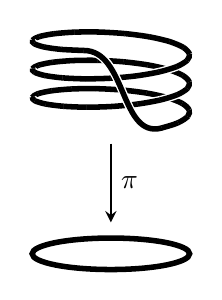
\begin{tikzpicture}[declare function={f(\x)=0.2*sin(\x)+\x/1000;},
  rubout/.style={/utils/exec=\tikzset{rubout/.cd,#1},
  decoration={show path construction,
       curveto code={
        \draw [white,line width=\pgfkeysvalueof{/tikz/rubout/line width}+2*\pgfkeysvalueof{/tikz/rubout/halo}] 
         (\tikzinputsegmentfirst) .. controls
         (\tikzinputsegmentsupporta) and (\tikzinputsegmentsupportb)  ..(\tikzinputsegmentlast); 
        \draw [line width=\pgfkeysvalueof{/tikz/rubout/line width},shorten <=-0.1pt,shorten >=-0.1pt] (\tikzinputsegmentfirst) .. controls
         (\tikzinputsegmentsupporta) and (\tikzinputsegmentsupportb) ..(\tikzinputsegmentlast);  
       }}},rubout/.cd,line width/.initial=2pt,halo/.initial=0.5pt]
  \draw[rubout={line width=2pt,halo=0.5pt},decorate] 
    plot[variable=\x,domain=-50:970,samples=55,smooth] ({cos(\x)},{f(\x)}) to[out=0,in=195] cycle;
  \draw[line width=2pt] (0,-2) arc(-90:270:1cm and 0.2cm);
  \draw[thick,-stealth]  (0,-0.4) -- (0,-1.4) node[midway,right]{$\pi$};
 \end{tikzpicture} 

There is no global section $s: S^1 \to X$ but locally, the set of sections $\{s: U \to \pi^{-1}(U) | \pi \circ s = id$ is a set with three elements.

Let $X$ be a topological space. A theorem of algebraic topology says that for any abelian group $A$, the cohomology group $H^1(X,A)$ with coefficients in $A$ is isomorphic to the abelianisation of the fundamental group $\pi_1(X)$